\documentclass[10pt,a4paper]{article}
\usepackage[utf8]{inputenc}
\usepackage[spanish]{babel}
\usepackage{amsmath}
\usepackage{amsfonts}
\usepackage{amssymb}
\usepackage{makeidx}
\usepackage{graphicx}
\usepackage{lmodern}
\usepackage{kpfonts}
\usepackage[left=2cm,right=2cm,top=2cm,bottom=2cm]{geometry}
\begin{document}
\begin{center}

\includegraphics[scale=0.2]{imagenes/upzmg.png} 
\end{center}
\paragraph{\Huge Simulacion de cinematica directa e inversa de manipuladores seriales.} \textbf{\Huge \\ \\ \\Integrates:} \\ \\
	\begin{Large}
		Samuel Caleb Martinez Hernandez\\ \\
		Fabian Canales Ochoa\\ \\
		Amaury Efrain Gutierrez Chavez\\ \\
		Cesar Fabian Flores Macias\\ \\
		\end{Large}
		\textbf{\Huge Materia:}\\ \\
		{\Large Cinemática de Robots}\\ \\
		\section{ \Huge Introduccion}
{\Large En esta practica se muestra la simulacion de la cinematica directa de nuestro diseño del robot scara.} \\ \\
\section{{\Huge Objetivo}}
{\Large Realizar la simulacion con ayuda de la convencion DENAVIT HARTENBERG.}\\ \\
\section{{\Huge Procedimiento}}
{\Large La primera parte fue enumerar los n + 1 eslabones de 0 a n, comnezando desde la basey terminando en el efector como se muestra en la imagen (1.1 , 1.2 Y 1.3).}\\ \\
\begin{center}
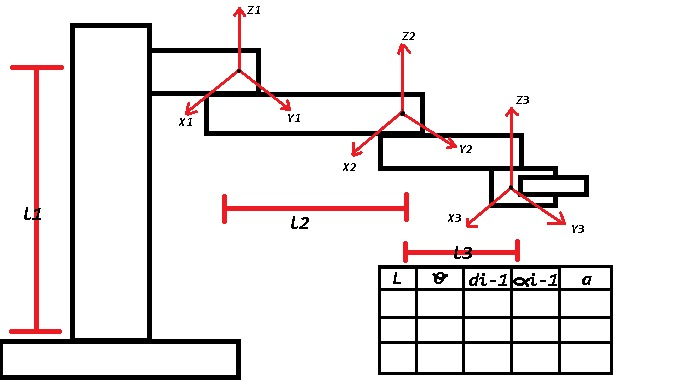
\includegraphics[scale=0.5]{imagenes/A.png} imagen 1.1  
\\{este es el diseño de nuestro robot y sus eslabones.} \\ 
\end{center}
\begin{center}
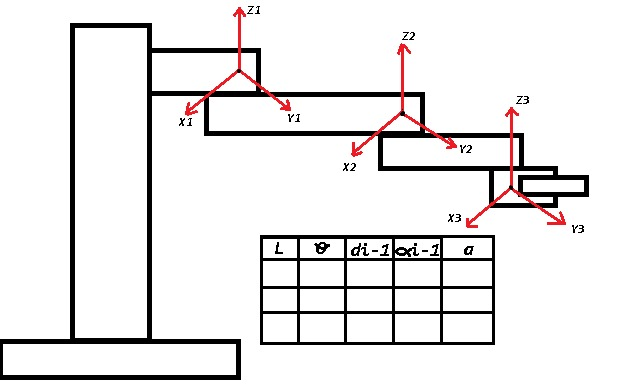
\includegraphics[scale=0.5]{imagenes/B.png} imagen 1.2  
\end{center}
\begin{center}
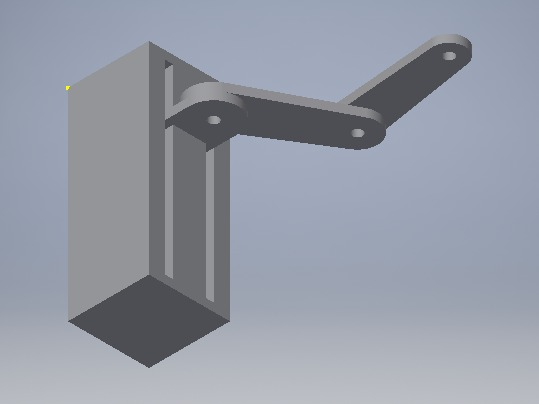
\includegraphics[scale=0.5]{imagenes/prototipo.png} imagen 1.3  
\\{este es el diseño de nuestro robot en 3D.} \\ 
\end{center}
{\Large Con los ejes definidos podemos comenzar a determinar los parametro con respectos a los angulos de desplazamiento y las distancias en las siguientes imagenes se muestra como fue que designamos valores  (imagenes 1.4, 1.5)

\begin{center}
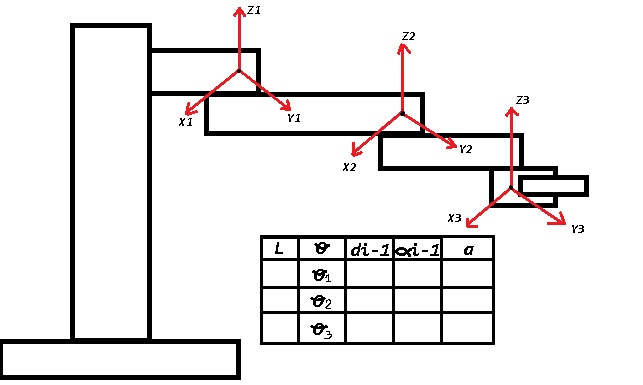
\includegraphics[scale=0.5]{imagenes/Z.png} imagen 1.4
\end{center}

\begin{center}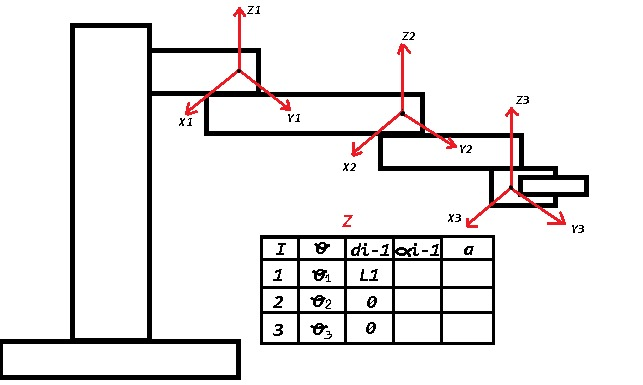
\includegraphics[scale=0.5]{imagenes/C.png} imagen 1.5
\end{center}
{\Large una vez que determinamos los parametros podemos realizar una matriz \textbf{D H} nuestra matriz quedo como se describe la imagen 1.6, 1.7 y 1.8
\begin{center}
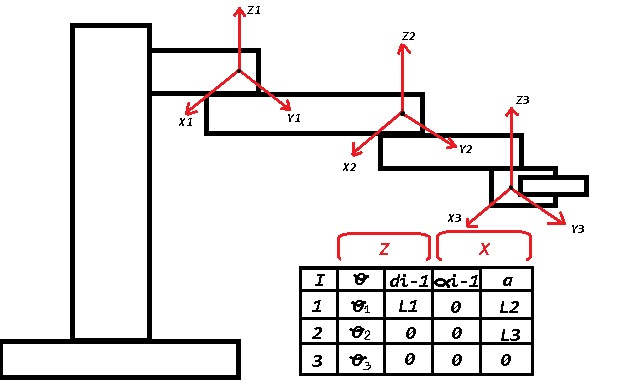
\includegraphics[scale=0.5]{imagenes/E.png} imagen 1.6
\end{center}
\begin{center}
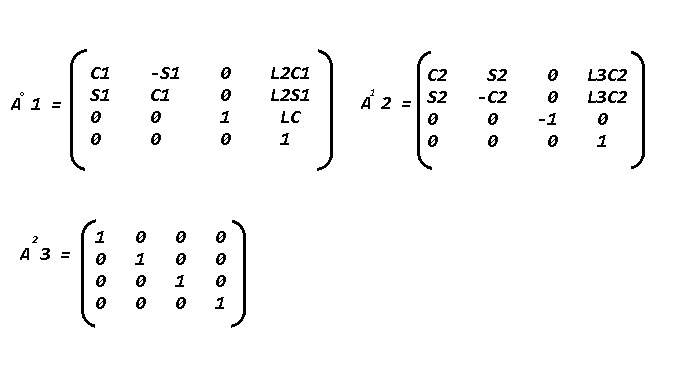
\includegraphics[scale=0.65]{imagenes/F.png} imagen 1.7 
\\ esta es la primera matriz que realizamos
\end{center}
\begin{center}
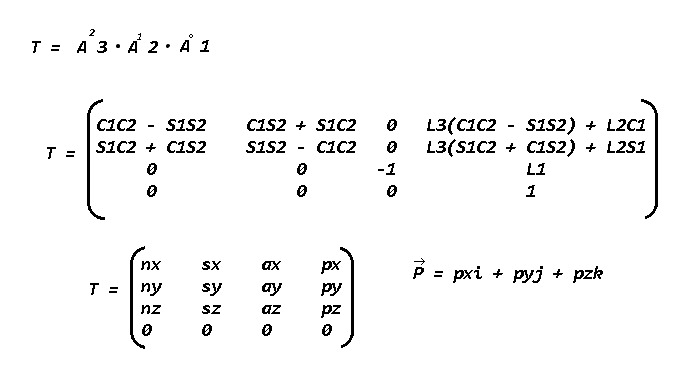
\includegraphics[scale=0.5]{imagenes/G.png} imagen 1.8 
\\ y esta es la matriz homogenea con los paramtros de nuestro robot
\end{center}

\section{{\Huge Conclusiones }}
{\large \huge\textbf{ Fabian Canales Ochoa}  este es un buen metodo de realizar matrices y tener conocimientos de el metodo de Denavit no es un tema que domine al cien por ciento pero nos ayuda a darnos una guia de los movimientos denuestro robots para el momento de montar los motores no este con movimientos forzados y no maltrate el materila del robot y que no le de mas carga a los motores .\\ \\ \\
{\large \huge\textbf{ Cesar Fabian Flores Macias}
El movimiento de los brazos robóticos no es tan secillo como uno puede suponer, ya que involucra no solo cálculos matemáticos, sino que se deben tener en cuenta parámetros específicos como la medidas de cada pieza a utilizar en e robot, también saber con realizar las matrices de denavit-Hasemberg para que el robot haga lo posible por replicar el movimiento o acción a realizar por el usuario.\\ 

{\large \huge\textbf{ Samuel Caleb Martinez Hernandez}	
LPese a que tomamos en cuenta de manera gráfica los tres ángulos x y z, es mucho menos confuso si se colocan solo dos ángulos a estudio y análisis, dado que el tercero suele ser irrelevante, aún así, está práctica se prestó para conocer a fondo la cinemática de nuestro robot.\\ 

{\large \huge\textbf{ Amaury Efrain Gutierrez Chavez}
Para mi este es solo una pequeña parte solamente es el diseño del robot hay una resistir los motores que sean mejores para que asi cumpla con los tres grados de libertad y que no se deforme el robot.
	
\paragraph{\Huge Referencias}\\ \\

Barrientos, A., Álvarez, M., Hernández, J. D., Del Cerro, J., & Rossi, C. (2012). Modelado de Caden as Cinemáticas mediante Matrices de Desplazamiento. Una alternativa al método de Denavit-Hartenberg. Revista Iberoamericana de Automática e Informática industrial, 9(4), 371-382.	

\end{document}